\subsubsection{Supervised Text Generation Tasks}
\label{appendix-subsec:standard-tasks}

Finally, we conduct experiment on standard generation tasks where clean supervised data is available. The study is to examine the capabilities of the proposed RL method to train a text generation model \emph{from scratch}, which has been considered as exceedingly challenging for previous RL algorithms.



\begin{table}
\centering
\small
\begin{tabular}{@{}l|llll@{}}
\toprule
\textbf{Model} & MLE & PG & MLE+PG & SQL (ours) \\
\midrule
\textbf{val} & $45.67$ & $0.00$ & $49.08$ & $47.04$ \\
\textbf{test} & $41.75$ & $0.00$ & $42.26$ & $41.70$ \\
\bottomrule
\end{tabular}
\vspace{-5pt}
\caption{BLEU results on the E2E val/test sets.}
\label{table:e2e-results}
\end{table}


\paragraph{Setup.}
We study on two tasks, E2E \citep{novikova2017e2e} and CommonGEN \citep{lin-etal-2020-commongen}, and use the respective datasets pre-processed by \citep{gehrmann2021gem} which allow sequence-to-sequence modeling with standard transformers.
We run four sets of methods:
the standard MLE training (\texttt{MLE}); PG training from scratch (\texttt{PG}); joint MLE and PG training, with MLE initialization (\texttt{MLE+PG}); and our SQL training from scratch with both off-policy and on-policy updates (\texttt{SQL}). We use the standard BLEU as reward.
We additionally investigate the training stability and sensitivity w.r.t hyperparameters, in particular the scale of reward. To this end, for \texttt{MLE+PG} and \texttt{SQL}, we vary the reward scale in $\{1, 10, 50, 100, 500, 1000\}$ and evaluate the respective performance under different scales.


\begin{figure*}
    \centering
    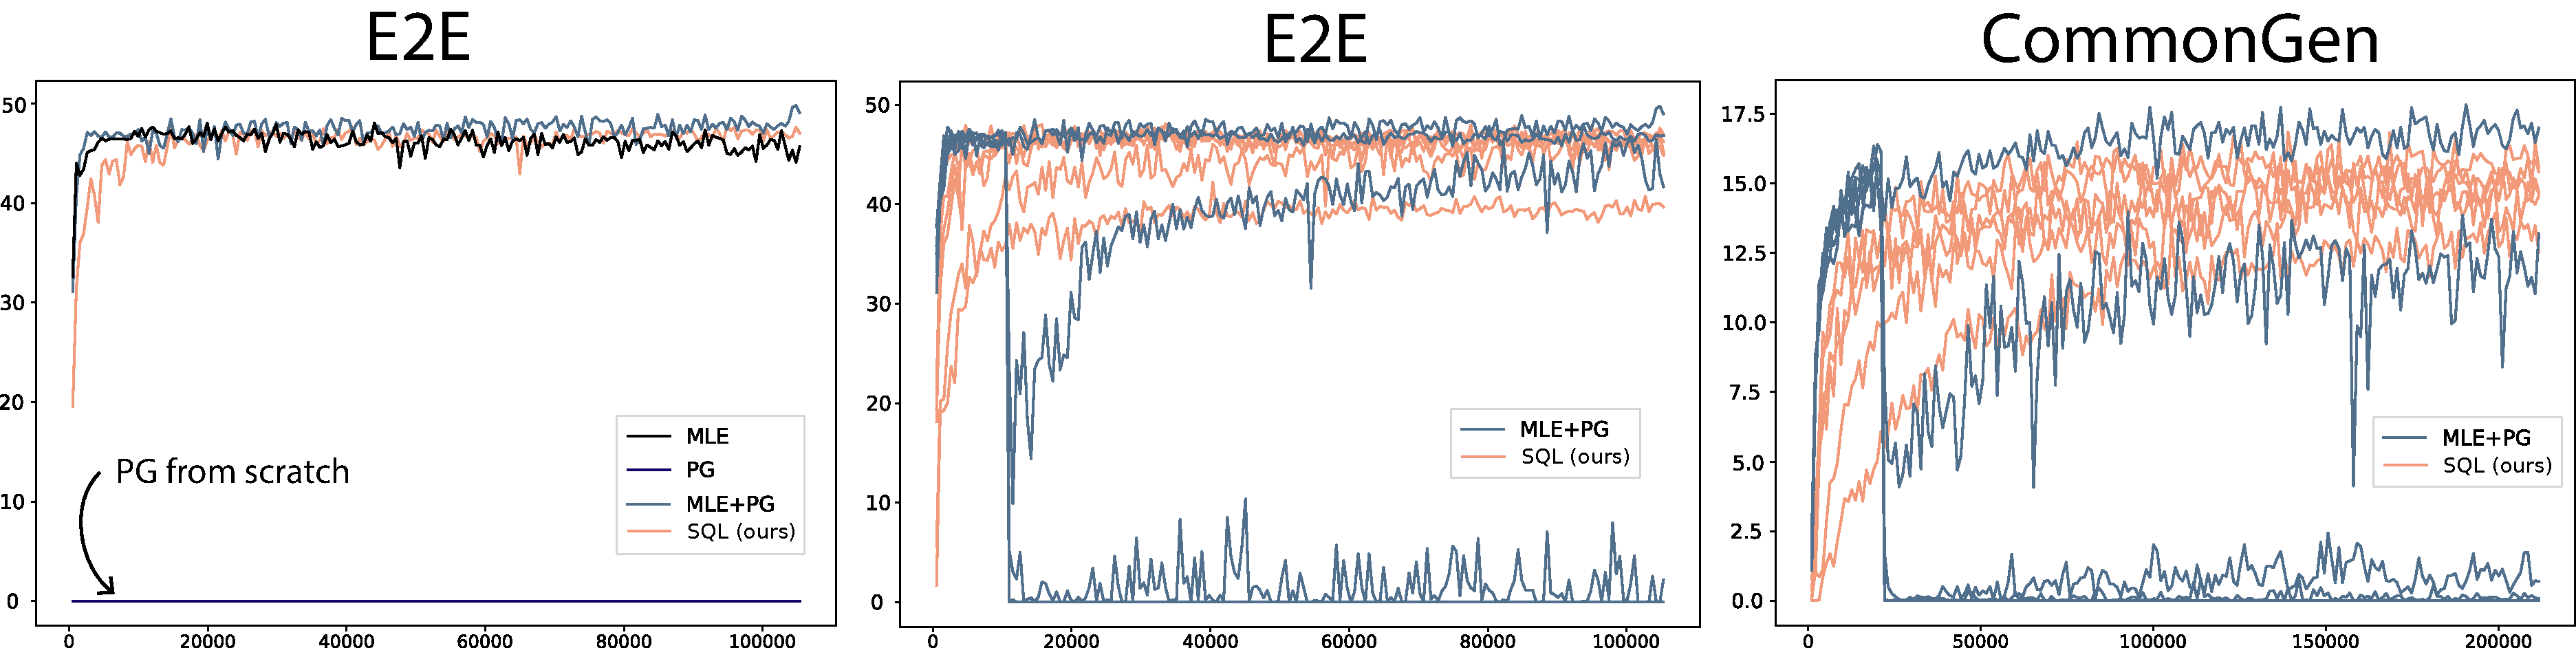
\includegraphics[width=0.99\linewidth]{figures/20210530.standard-tasks-small.pdf}
    \caption{Training curves on validation sets. {\bf Left:} Training curves on E2E with best hyperparameter configurations. {\bf Middle:} Training curves on E2E with varying reward scale. {\bf Right:} Training curves on CommonGen with varying reward scale.
    }
    \label{fig:supervised-text-generation-tasks}
\end{figure*}

\paragraph{Results.}
Table~\ref{table:e2e-results} shows the performance on E2E of different models whose hyperparameters are picked using the validation set. We can see the proposed \texttt{SQL} that trains models from scratch achieves competitive results with the common \texttt{MLE} and \texttt{MLE+PG}. In contrast, the \texttt{PG} algorithm alone without MLE fails the training. Figure~\ref{fig:supervised-text-generation-tasks} (left) shows the respective training curves (on the validation set), demonstrating that \texttt{SQL} converges in an efficient and stable way as \texttt{MLE}.

We further demonstrate the sensitive of \texttt{MLE+PG} and \texttt{SQL} w.r.t the reward scale as a key hyperparameter. Figure~\ref{fig:supervised-text-generation-tasks} (middle and right) shows the training curves of the two methods with varying reward scales. We can see \texttt{SQL} is significantly more robust as reward scale changes, while \texttt{MLE+PG} tends to collapse with improper reward scale configurations. 


